\newpage
\section{Специальная часть}
\subsection{Обратная динамика}
\pagestyle{fancy}
\fancyhf{}
\rhead{Дипломная работа}
\lhead{Специальная часть}
\rfoot{\thepage}

Чтобы улучшить пилотажные характеристики и точность пилотирования, возможно синтезировать контроллер на основе 
принципа обратной динамики, который показан в работе {\cite{Zoe}}. Но при использовании данного метода порядок числителя будет выше порядка знаменателя, поэтому необходимо использовать фильтры.

В этой работе мы будем вычислять обратную динамику с помощью обратных связей, т.к. здесь нет необходимости ставить дополнительные фильтры.

\subsection{Исслеуемая модель}
\subsubsection{Модель самолёта}

Данная модель была всзята из дисертации {\cite{Diser}}

Основные допущения: 
\begin{enumerate}
    \item Рассмотривается линеаризованная модель короткопериодического движения 
    \item Система исследуется в продольном канале управления
    \item Угол атаки $\alpha$ постоянный и равен $13,7^0$ 
\end{enumerate}

Линейная математическая модель может быть представлена в знакомой форме пространства состояний в виде:
\begin{equation}
    \begin{aligned}
        \dot{x}(t) = Ax(t) + Bu(t) \\
        y(t) = Cx(t) + Du(t)
    \end{aligned}
\end{equation}

Линейная математическая модель может быть представлена в знакомой форме пространства состояний в виде:

\begin{equation}
    \label{eq:Линеаризованная моель СПС}
\begin{bmatrix}
        \dot{V}_x\\ 
        \dot{V}_y\\ 
        \dot{\omega_z}\\ 
        \dot{\theta}
    \end{bmatrix} =
    \begin{bmatrix}
        -0.0110 & 0.0433 & 1.7295 & -7.1876\\ 
        -0.0691 & -0.6975 & -7.0678 & -54.8976\\ 
        0.00011 & 0.00116 & -0.35407 & 0.0911\\ 
        0 & 0 & 1 & 0
    \end{bmatrix} \begin{bmatrix}
        V_x\\ 
        V_y\\ 
        \omega_z \\ 
        \theta
    \end{bmatrix} 
        +\begin{bmatrix}
        -0.4412\\ 
        -12.388\\ 
        -0.58446 \\ 
        0
    \end{bmatrix}  u
\end{equation}

Система ДУ приводит к следующей краткой аэродинамической и управляющей производной:

\begin{equation}
    \label{eq:Линеаризованная моель СПС}
\begin{bmatrix}
        \dot{V}_x\\ 
        \dot{V}_y\\ 
        \dot{\omega_z}\\ 
        \dot{\theta}
    \end{bmatrix} =
    \begin{bmatrix}
        x_{V_x}& x_{V_y}&x_{\omega_z} &x_{\theta} \\ 
        z_{V_x}&z_{V_w} &z_{\omega_z} &z_\theta \\ 
        m_{V_x}&m_{V_y} &m_{\omega_z} &m_\theta \\ 
        0& 0& 1&0 
    \end{bmatrix} \begin{bmatrix}
        V_x\\ 
        V_y\\ 
        \omega_z \\ 
        \theta
    \end{bmatrix} 
        +\begin{bmatrix}
        x_{\delta_\text{э}}\\ 
        z_{\delta_\text{э}}\\ 
        m_{\delta_\text{э}}\\ 
        0
    \end{bmatrix} \delta_\text{э} 
\end{equation}

Относительные величины и знаки кратких аэродинамических
производных относительного момента тангажа, $m_{V_x}$, $m_{V_y}$, $m_{\omega_z}$ и $m_\theta$, важны для устойчивости и динамических свойств
самолета. Отмечая следующее:
\begin{itemize}
\item Член производной относительной момента по скорости, $m_{V_x}$, положительный из-за того, что центральная линия тяги расположена
ниже вертикального положения центра тяжести. Однако он очень мал (0,00011) и поэтому мало повлияет на стабильность системы.
\item Момент относительной производной по вертикальной скорости, $m_{V_y}$ хотя и небольшая, является положительной, что указывает на статически
неустойчивый самолет.
\item Величина производной относительного демпфирующего момента, $m_{\omega_z}$, невелика, хотя и отрицательна и стабилизирует систему.
\end{itemize}

Входная матрица преобразует отрицательный (вверх) входной сигнал элевона в положительный момент шага, нормальную и осевую силу.

\subsubsection{Модель самолёт-лётчик}

Значительно сложнее выполнение задач точного пилотирования, представляющего собой процесс непрерывного взаимодействия лётчика
с объектом управления происходящей в замкнутой системе самолёт-лётчие (рис.{\ref{fig:Самолёт-лётчик}}).

\begin{figure}[H]
    \center{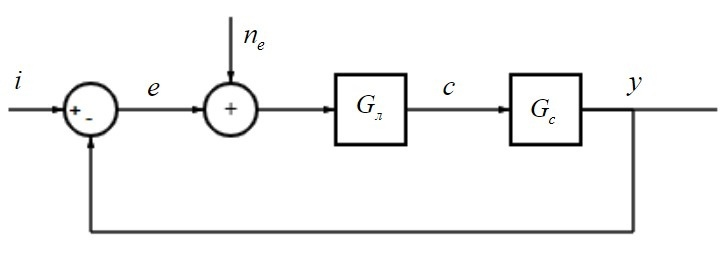
\includegraphics[width = \linewidth]{Оглавление/Part3/figures/СамолётЛётчик.png}}
    {\label{fig:Самолёт-лётчик}}
    \caption{Структурная схема системы самолёт-лётчик}   
\end{figure}

$W_\text{л} - $  Передаточная функция лётчика
$W_\text{с} - $  Передаточная функция объекта управления  

\subsubsection{Передаточные функции систему ДУ}

Зная систему дифференциальных уравнений ({\ref{eq:Линеаризованная моель СПС}}), найдём передаточные функции 

\begin{equation}
    \label{eq:ПФ по горизонтальной скорости СПС}
    \{ \frac{V_x}{\delta_\text{э}} \} = \frac{-0.4412p^3 - 2,011p^2 + 3.388p + 4.471}{p^4 + 1.063p^3 + 0.1784p^2 + 0.003833p + 3.424 \cdot 10^{-5}}
\end{equation}

\begin{equation}
    \label{eq:ПФ по вертикальной скорости СПС}
    \{ \frac{V_y}{\delta_\text{э}} \} = \frac{-12.39^3 - 0.3612p^2 + 33.29p + 0.06517}{p^4 + 1.063p^3 + 0.1784p^2 + 0.003833p + 3.424 \cdot 10^{-5}}
\end{equation}

\begin{equation}
    \label{eq:ПФ по угловой скорости тангажа СПС}
    \{ \frac{\omega_z}{\delta_\text{э}} \} = \frac{-0.5845p^3 - 0.4285p^2 - 0.006449p - 3.57 \cdot 10^{-20}}{p^4 + 1.063p^3 + 0.1784p^2 + 0.003833p + 3.424 \cdot 10^{-5}}
\end{equation}

\begin{equation}
    \label{eq:ПФ по углу наклона траектории}
    \{ \frac{\theta}{\delta_\text{э}} \} = \frac{-0.5845p^2 - 0.4285p - 0.006449}{p^4 + 1.063p^3 + 0.1784p^2 + 0.003833p + 3.424 \cdot 10^{-5}}
\end{equation}

\subsection{План исследований}
\subsubsection{Обратная динамики }
Обратная динамика вычислена через обратные связи как показанно на рис.\ref{fig:САУ_ОД}
\begin{figure}[H]
    \centering 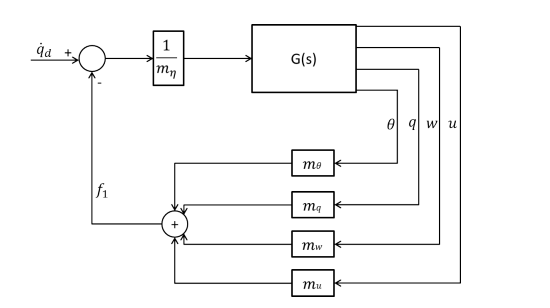
\includegraphics[width=15cm,height=10cm]{Оглавление/Part3/figures/САУ_ОД.png}
    \caption{Реализация динамической инверсии}
    {\label{fig:САУ_ОД}}
    \end{figure}
\subsection{Изучение робастности} 

Чтобы изучать робастность контроллера на основе обратной динамики, мы проводили  с разными моделями продольного движения разных самолётов. 

\subsubsection{Модель (European SPS)} 
    \begin{bmatrix}
        -0.0110 & 0.0433 & 1.7295 & -7.1876\\ 
        -0.0691 & -0.6975 & -7.0678 & -54.8976\\ 
        0.00011 & 0.00116 & -0.35407 & 0.0911\\ 
        0 & 0 & 1 & 0
    \end{bmatrix} \cdot X=\begin{bmatrix}
        -0.4412\\ 
        -12.388\\ 
        -0.58446 \\ 
        0
    \end{bmatrix} \cdot U=\dot{X}
\begin{center}
    Эксперименты с изменениями А и В
\end{center}

Суть данного эксперимента заключается в проверке характеристик надежности системы при изменении матрицы входных параметров $B$. Результаты эксперимента можно кратко изложить ниже.
    
\begin{figure}[H]
    \centering 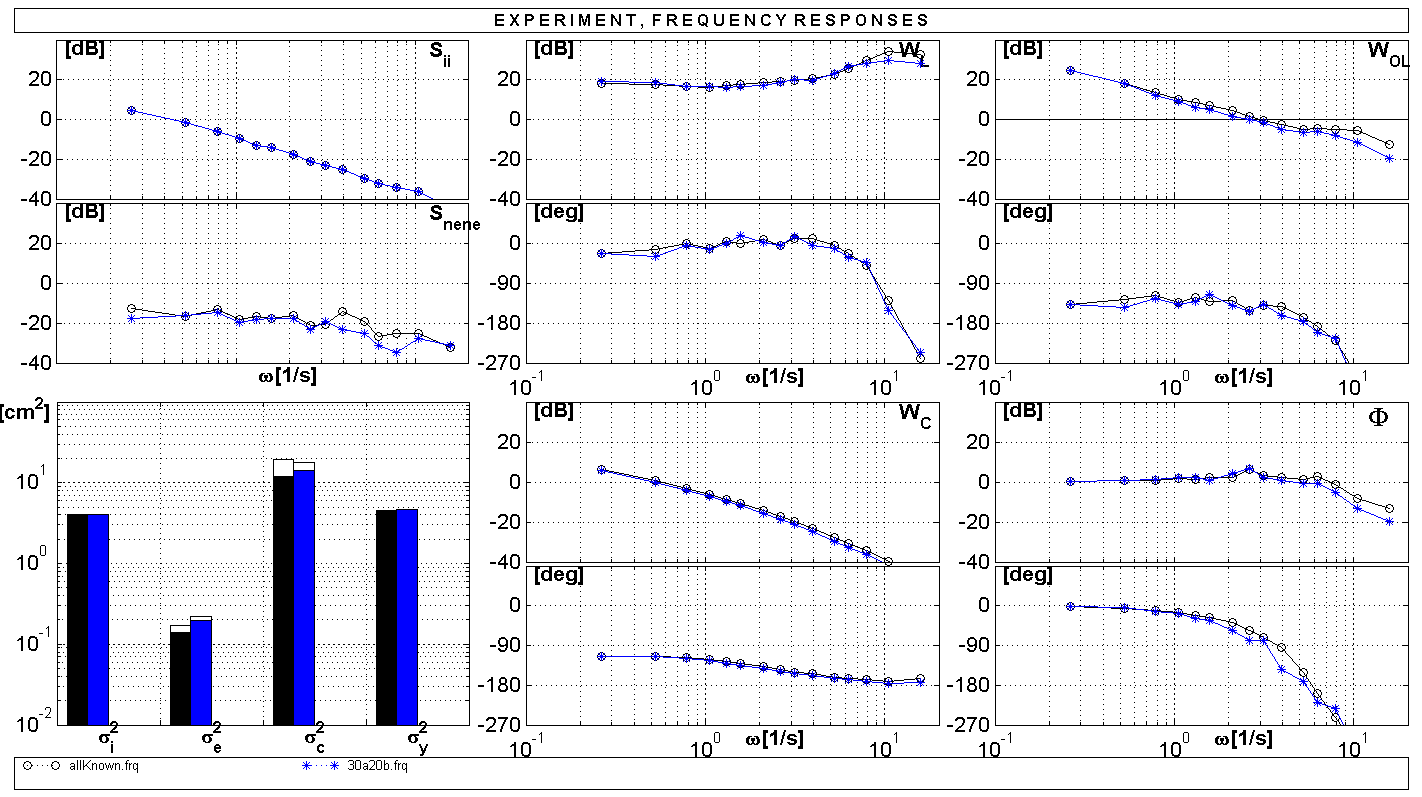
\includegraphics[width=17cm,height=15cm]{Оглавление/Part3/figures/chast2_20A30B.png}
    \caption{}
    {\label{fig:Частотки второй Системы с изменением А и В}}
    \end{figure}

    \begin{center}
        Эксперимент без PI 
    \end{center}



    Также мы подразумеваем, что мы имеем дело с $K_\text{ш} = -0,6$

    Из Рис. {\ref{fig:Результаты экспериментов без PI}}
    \begin{itemize}
        \item [-] c увеличением неточности знаний увеличивается $\sigma_e^2$
        \item [-] лётчик вводит меньшие усилия на ручку управления $\sigma^2_c$ 
        \item [-]  Я ещё ничего не приумал   
    \end{itemize}